% utf-8 ru, unix eolns
\documentclass[12pt,a4paper,oneside]{extarticle}
    \righthyphenmin=2 %минимально переносится 2 символа %%%
    \sloppy

% Рукопись оформлена в соответствии с правилами оформления 
% электронной версии авторского оригинала, 
% принятыми в Издательстве МГТУ им. Н.Э. Баумана.

\usepackage{geometry} % А4, примерно 28-31 строк(а) на странице 
    \geometry{paper=a4paper}
    \geometry{includehead=false} % Нет верх. колонтитула
    \geometry{includefoot=true}  % Есть номер страницы
    \geometry{bindingoffset=0mm} % Переплет    : 0  мм
    \geometry{top=20mm}          % Поле верхнее: 20 мм
    \geometry{bottom=25mm}       % Поле нижнее : 25 мм 
    \geometry{left=25mm}         % Поле левое  : 25 мм
    \geometry{right=25mm}        % Поле правое : 25 мм
    \geometry{headsep=10mm}  % От края до верх. колонтитула: 10 мм
    \geometry{footskip=20mm} % От края до нижн. колонтитула: 20 мм 

\usepackage{cmap}
\usepackage[T2A]{fontenc} 
\usepackage[utf8x]{inputenc}
\usepackage[english,russian]{babel}
\usepackage{misccorr}

\usepackage{amsmath}
\usepackage{amsfonts}
\usepackage{amssymb}

%\usepackage{cm-super} %человеческий рендер русских шрифтов

\setlength{\parindent}{1.25cm}  % Абзацный отступ: 1,25 см
\usepackage{indentfirst}        % 1-й абзац имеет отступ

\usepackage{setspace}   

\onehalfspacing % Полуторный интервал между строками

\makeatletter
\renewcommand{\@oddfoot }{\hfil\thepage\hfil} % Номер стр.
\renewcommand{\@evenfoot}{\hfil\thepage\hfil} % Номер стр.
\renewcommand{\@oddhead }{} % Нет верх. колонтитула
\renewcommand{\@evenhead}{} % Нет верх. колонтитула
\makeatother

\usepackage{fancyvrb}


\usepackage[pdftex]{graphicx}  % поддержка картинок для пдф
\graphicspath{ {./pictures/} }
\usepackage{rotating}
%\DeclareGraphicsExtensions{.jpg,.png}




\renewcommand{\labelenumi}{\theenumi.} %меняет вид нумерованного списка

\usepackage{perpage} %нумерация сносок 
\MakePerPage{footnote}

\usepackage[all]{xy} %поддержка графов

\usepackage{listings} %листинги


\usepackage{url}


\usepackage{tikz} %для рисования графиков
\usepackage{pgfplots}


\usepackage{ccaption}%изменяет подпись к рисунку
\makeatletter 
\renewcommand{\fnum@figure}[1]{Рисунок~\thefigure~---~\sffamily}
\makeatother

\begin{document}
\pgfplotsset{compat=1.8}

\thispagestyle{empty}
\newpage
{
\centering


\textbf{
МОСКОВСКИЙ ГОСУДАРСТВЕННЫЙ ТЕХНИЧЕСКИЙ УНИВЕРСИТЕТ ИМЕНИ Н. Э. БАУМАНА \\
Факультет информатики и систем управления \\
Кафедра теоретической информатики и компьютерных технологий}
\bigskip
\bigskip
\bigskip
\bigskip
\bigskip
\bigskip
\bigskip

\vfill


Курсовой проект \\
по курсу <<Компьютерные системы и сети>>

\bigskip

{\large <<Фреймворк и файловая система для распределённой обработки больших данных в рамках концепции map-reduce>>}
\bigskip

\vfill



\hfill\parbox{4cm} {
Выполнил:\\
студент ИУ9-91 \hfill \\
Выборнов А. И.\hfill \medskip\\
Руководитель:\\
Дубанов А. В.\hfill
}


\vspace{\fill}

Москва \number\year
\clearpage
}


\tableofcontents

\clearpage


\section*{Введение}
\addcontentsline{toc}{section}{Введение}
   С каждом годом объём данных, которые необходимо обрабатывать, растёт, что привело к появлению термина {\it большие данные} и развитию инфраструктуры по их обработке. Обработка больших данных достаточно молодая и динамично развивающаяся отрасль ИТ.

   В ходе данной работы были разработаны и реализованы фреймворк, который позволяет обрабатывать большие данные с использованием концепции map-reduce, и распределённая файловая система, обеспечивающая функционал, необходимый для работы фреймворка.
\clearpage

\section{Теоретическая часть}
    \subsection{Map-reduce}
        {\it Map-reduce} --- концепция, используемая для распределённых вычислений над {\it большими данными} в компьютерных кластерах. Модель представлена компанией Google в 2004 году~\cite{mapreduce}.

        {\it Большие данные~(Big data)} --- термин, характеризующий любой набор данных, который достаточно велик и сложен для традиционных методов обработки, а также набор технологий для работы с такими данными.
        
        Выполнение приложения в рамках концепции map-reduce состоит из двух последовательных этапов, между которыми происходит группировка результатов:
        \begin{itemize}
            \item $map$ --- предварительная обработка входных данных,
            \item $reduce$ --- свёртка предварительно обработанных данных.
        \end{itemize}

        Несмотря на то, что прототипами этапов $map$ и $reduce$ послужили одноимённые функции, используемые в функциональном программировании,~---~их семантика заметно отличается.

        Базовым элементом в концепции map-reduce является структура (key, value) --- (ключ, значение). Программирование представляет собой определение двух функций (квадратные скобки [~] обозначают список):
        \begin{itemize}
            \item $map: (key, value)\rightarrow[(key, value)]$
            \item $reduce: (key, [value])\rightarrow[(key, value)]$
        \end{itemize}

        Приведённое выще определение является достаточно абстрактным для прикладного применения. На практике достаточно следующего варианта выше приведённого определения:
        \begin{itemize}
            \item $map: $~файл ввода~$\rightarrow[(key, value)]$
            \item $reduce: (key, [value])\rightarrow$~файл вывода
        \end{itemize}

        \begin{figure}[h!]
            \centering
            
\includegraphics[scale=0.7]{mapreduce.png}
            \caption{Схематическое изображение обработки данных с помощью концепции map-reduce}
            \label{pic:mapreduce}
        \end{figure}

        На рисунке~\ref{pic:mapreduce} схематически изображена обработка данных с помощью map-reduce. Файл ввода разбивается на блоки, каждый из которых поступает на вход функции $map$. Функция map обрабатывает его и порождает список пар (ключ, значение). Множество полученных списков пар объединяется и группируется по ключу, получая пары вида (ключ, список значений). Все пары равномерно распределяются на блоки и передаются на вход стадии $reduce$. Стадия $reduce$ преобразовывает ключ и список значений в блок, являющийся частью файла вывода.

        Как видно из описания, концепция налагает ограничения на формат файлов ввода и вывода: данные должны быть коммуникативны, с некоторой точностью (обычно до строки).

        \subsubsection{Проблемы, которые решаются с помощью map-reduce}
            Концепция map-reduce, довольно быстро обрела популярность, так как накопилось множество проблем, не имеющих универсального решения~\cite{problem}. Вот основные из них~(в скобках указан подход к решению используемый в концепции map-reduce):

            \begin{itemize}
                \item вычисления превосходят возможности одной машины~(кластеры из сотен и тысяч машин),
                \item данные не помещаются в памяти, необходимо обращаться к диску~(последовательное чтение и запись намного эффективнее случайного доступа),
                \item большое количество узлов в кластере вызывает множество отказов~(все узлы унифицированы, что упрощает восстановление работы после отказа),
                \item данные хранятся на множестве машин~(данные обрабатываются на той же машине, на которой они хранятся),
                \item достаточно дорогая и сложная разработка низкоуровневных приложений для подобных систем~(высокоуровневая модель программирования, универсальная и масштабируемая среда выполнения).
            \end{itemize} 

        \subsubsection{Пример применения map-reduce}

            {\bfЗадача:} Есть граф пользователей некоторого ресурса, заданный в виде пар (пользователь, <<друг$_1$ друг$_2$ ...>>). Для каждой пары пользователей найти общих друзей.

            Разбор решения задачи будет проводится для следующих входных данных: 
            \lstset{}
            \begin{lstlisting}[mathescape] 
    (A, B C D)
    (B, A C)
    (C, A B D)
    (D, A C)
            \end{lstlisting}

            Пусть функция map преобразовывает пару (пользователь, друзья) в множество пар.
            Для каждого друга формируется пара (ключ, значение) следующим образом: ключ~---~строка <<пользователь друг>>, если строка <<пользователь>>~$>$~строки <<друг>>, иначе строка <<друг пользователь>>, значение~---~<<друзья>>. Выполнения функции map в формате (входные даннные $\rightarrow$ результат):

            \lstset{}
            \begin{lstlisting}[mathescape] 
    (A, B C D) $\rightarrow$ [(A B, B C D), (A C, B C D), (A D, B C D)]
    (B, A C) $\rightarrow$ [(A B, A C), (B C, A C)]
    (C, A B D) $\rightarrow$ [(A C, A B D), (B C, A B D), (C D, A B D)]
    (D, A C) $\rightarrow$ [(A D, A C), (C D, A C)]
            \end{lstlisting}
                
            По выполнении функции map происходит подготовка данных для функции reduce, множество полученных пар агрегируется по ключу:

            \lstset{}
            \begin{lstlisting}[mathescape] 
    (A B, [B C D, A C])
    (A C, [B C D, A B D])
    (A D, [B C D, A C])
    (B C, [A B D, A C])
    (C D, [A B D, A C])
            \end{lstlisting}

            Функция reduce пересекает все элементы списка значений. Выполнение функции reduce в формате (входные даннные $\rightarrow$ результат):

            \lstset{}
            \begin{lstlisting}[mathescape] 
    (A B, [B C D, A C]) $\rightarrow$ (A B, C)
    (A C, [B C D, A B D]) $\rightarrow$ (A C, B D)
    (A D, [B C D, A C]) $\rightarrow$ (A D, C)
    (B C, [A B D, A C]) $\rightarrow$ (B C, A)
    (C D, [A B D, A C]) $\rightarrow$  (C D, A)
            \end{lstlisting}


        По выполнении функции reduce получили множество пар (ключ значение), где ключ~---~пара пользователей, значение~---~множество общих друзей:

            \lstset{}
            \begin{lstlisting}[mathescape] 
    (A B, C)
    (A C, B D)
    (A D, C)
    (B C, A)
    (C D, A)
            \end{lstlisting}

    \subsection{Распределённая файловая система}
        {\it Распределённая файловая система~(РФС)}~---~файловая система, в которой данные хранятся на нескольких узлах. 

        При реализации фреймворка map-reduce РФС требуется для хранения одного файла в виде набора блоков, распределённых по нескольким узлам, а также для создания файла из блоков данных, расположенных на нескольких машинах.

        Распределённая файловая система является вспомогательным компонентом, поверх которого работает map-reduce. В рамках данной работы рассматривалась упрощенная модель файловой системы, которая обеспечивает все потребности map-reduce, но при этом не обладает некоторыми важными возможностями файловых систем, такими как расширенные характеристики файлов и реплицируемость.

        В рамках работы была разработана РФС, которая позволяет хранить файлы, упорядоченные с помощью древовидной структуры каталогов. Файл представляет собой именованную последовательность блоков данных, которые распределены по нескольким узлам. Файл бьётся на блоки равного размера~(64 Мбайт) с точностью до переносов строк.

        \begin{figure}[h!]
            \centering
            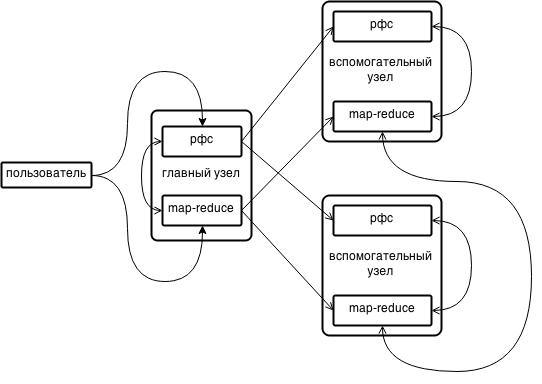
\includegraphics[scale=0.75]{framework_total.png}
            \caption{Взаимосвязь узлов при работе фреймворка map-reduce}
            \label{pic:framework}
        \end{figure}
        
        На рисунке~\ref{pic:framework} показана общая архитектура фреймворка map-reduce. Рассмотрим часть, связанную с РФС.
        Пользователь работает с элементом РФС расположенном на главном узле, на котором хранится структура файловой системы и информация о блоках, составляющих каждый файл.
        Вспомогательные узлы хранят блоки и имеют интерфейс, позволяющий создавать, получать, удалять и переименовывать блоки.
    \subsection{Распределённый map-reduce}
        Рассмотрим рисунок~\ref{pic:framework}. Пользователь работает с интерфейсом map-reduce на главном узле. Map-reduce на главном узле занимается управлением процессом выполнения задачи, может взаимодействовать с РФС на главном узле, а также с map-reduce на дочерних узлах. Map-reduce на дочерних узлах выполняет код функций map и reduce, а также записывает и читает данные, взаимодействуя с элементом РФС на дочернем узле.

        Выполнение программы с помощью фреймворка map-reduce происходит следующим образом:
        \begin{enumerate}
            \item На вход подаются адреса файлов из РФС, для ввода и вывода, и файл с функциями map и reduce.
            \item Из РФС получается список индексов, соответствующий файлу ввода.
            \item Полученный список индексов группируется по узлам.
            \item Каждому дочернему узлу сообщается о начале стадии map: передаётся соответствующий ему список индексов и файл с функциями map и reduce.
            \item Выполняется стадия map на дочерних узлах. Стадия map порождает данные, равномерно распределяющиеся по дочерним узлам.
            \item Каждому дочернему узлу сообщается о начале стадии reduce.
            \item Выполняется стадия reduce на дочерних узлах. Стадия reduce порождает множество блоков, задаёт им псевдоимена и сообщает об этом главному узлу.
            \item Главный узел производит переименование блоков путём задания им новых имён и записывает информацию о файле вывода в РФС.
        \end{enumerate}
        
        \begin{sidewaysfigure}
            \centering
            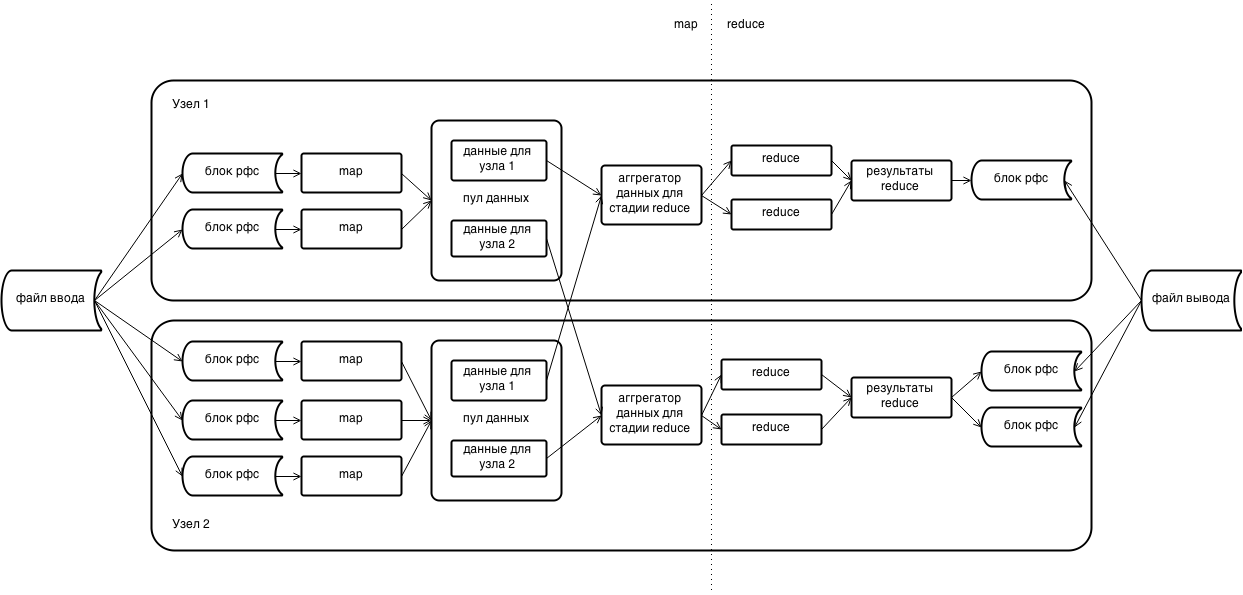
\includegraphics[scale=0.55]{map_reduce_framework.png}
            \caption{Схема выполнения приложения с помощью фреймворка map-reduce}
            \label{pic:mr_framework}
        \end{sidewaysfigure}

        На рисунке~\ref{pic:mr_framework} показано выполнение стадий map и reduce~(отделены пунктиром) на двух узлах. Выполнение стадий происходит следующим образом:
        \begin{itemize}
            \item Стадия map.
            \begin{enumerate}
                \item Для каждого блока РФС, соответствующего полученному индексу, выполняется функция map. Блоки обрабатываются последовательно.
                \item Во время обработки блока все результаты попадают в пул данных, где распределяются по дочерним узлам.
                \item По окончании обработки блока пул данных рассылает полученные результаты по соответствующим дочерним узлам.
                \item Результаты агрегируются на узлах в оперативной памяти.
            \end{enumerate}
            \item Стадия reduce.
            \begin{enumerate}
                \item Для каждой пары (ключ, список значений) выполняется функция reduce.
                \item Результаты выполнения функции reduce агрегируются в оперативной памяти.
                \item По завершении обработки всех данных результат преобразуется в текст, который разбивается на блоки фиксированного размера~(64 Мбайт).
                \item Полученные блоки записываются в РФС.
            \end{enumerate}
        \end{itemize}
        


    \subsection{Решаемый класс задач}
    \label{sec:tasks}
        Необходимо обосновать существование и найти класс задач (здесь и далее под классом подразумевается некоторое множество задач), для которого актуальна приведённая выше схема распределённого map-reduce.

        Пусть каждый узел располагает $memory$ доступной оперативной памяти (здесь и далее единицей измерения памяти будет байт) и $storageSize$ свободного места на диске. Всего узлов $numNodes$. Данный map-reduce проектировался для решения задач с {\it большими данными}, поэтому в дальнейшем будем считать, что входные данные $>>memory$. 

        \subsubsection{Oграничения на стадии map и reduce}
            На вход стадия map принимает данные с диска, а результат этой стадии равномерно (с точностью до пары (ключ, значение)) распределяется по оперативной памяти узлов. То есть входные данные $<storageSize*numNodes$, а результат $<< memory*numNodes$. Так как $storageSize >> memory$, получаем, что, в общем случае, стадия map должна сильно сокращать объём данных.

            На вход стадия reduce принимает данные из оперативной памяти, которые $<< memory*numNodes$, результат этой стадии аккумулируется в оперативной памяти, то есть должен быть $<<memory$ для каждого узла, а затем записывается на диск. Получаем, что стадия reduce должна, как минимум, не увеличивать объём данных, поступивших на вход.

            Рассмотрев полученные выше ограничения для стадий map и reduce, а также учитывая достаточно большие входные данные, можно увидеть, что распределённый map-reduce оптимально подходит для решения задач класса {\it информационный поиск} ({\it information retrieval}), что является одним из этапов решения задач {\it анализа данных} ({\it data mining}).

            {\it Информационный поиск} --- процесс поиска и получения информации как из структурированных, так и из неструктурированных данных. Обычно применяется в {\it анализе данных} для первичной обработки и сокращения объёма исходных данных~\cite{mr_tasks}. 

        \subsubsection{Пример задачи класса информационный поиск}
        \label{sec:task_example}
            Исходные данные хранятся в виде текстового файла в $n$ строк, в котором каждая строка соответствует строке в реляционной таблице $table$ с $m$ столбцов ($f_1...f_m, m>2$). Необходимо получить результат выполнения SQL запроса:
            \lstset{language=SQL}
            \begin{lstlisting}[mathescape] 
    SELECT $f_0, ..., f_m$
    FROM $table$
    WHERE $f_j > const$
            \end{lstlisting}
            и сгруппировать его по ключу $f_i$. В результате все строки с одинаковым $f_i$ должны идти одним непересекающимся блоком.

        \subsubsection{Решение задачи с помощью фреймворка map-reduce}
            
            Функция map определяется следующим образом: для каждой строки проверяется условие {\bf WHERE} и все строки, удолетворяющие условию, составляют результат в виде пар: $(f_i, f_1, ..., f_m)$. Количество строк, удолетворяющих условию {\bf WHERE}, обозначим как $n'$. Функция reduce возвращает список значений.

            Стадия map получает $O(nm)$ данных и, по выполнении, выдаёт $O(n'm)$ данных, которые преобразуются и без изменений проходят стадию reduce. Сложность стадии map~---~$O(nm)$, преобразования между стадиями~---~$O(n'm+n'ms_{net})$ ($s_{net}$~---~стоимость передачи данных между узлами), стадии reduce~---~$O(n')$. 

        \subsubsection{Решение задачи на одной машине}
            Решение задачи на одной машине без применения фреймворка состоит из двух стадий: 
            \begin{itemize}
                \item получить из входного файла все строчки, удолетворяющие {\bf WHERE}~---~сложность $O(nm)$ (по памяти $O(n'm)$),
                \item сгруппировать полученный результат по ключу $f_i$~---~сложность $O(n'ln(n'))$, если применить для агрегации быструю сортировку (по памяти $O(n'm)$), сложность $O(n')$, если применить для аггрегации сортировку подсчётом (по памяти $2O(n'm)$).
            \end{itemize}

            В случае когда $n'$ и $m$ определены таким образом, что получишиеся данные больше $memory$, возникают проблемы: необходимо сохранять на диск промежуточные результаты, полученные после первой стадии, и сортировать полученный результат на диске, что достаточно медленно. Рассмотрим вариант решения этих проблем: результат первой стадии разбивается на блоки, каждый из которых сортируется и сохраняется в файл, после обработки всех результатов полученные файлы сливаются). Сложность первой стадии~---~$O(nm+n'ln(n')+n's_{hdd})$, второй стадии $O(n'ms_{hdd})$ ($s_{hdd}$~---~стоимость обращения к диску).

        \subsubsection{Выводы}
            Cуммарная сложность решения с помощью map-reduce~---~$O(nm+n'm+n'ms_{net}+n')$, с помощью описанного выше способа решения на одной машине~---~$O(nm+n'ln(n')+n's_{hdd}+n'ms_{hdd})$. Можно увидеть, что по сложности данные алгоритмы принципиально не отличаются (в обоих случаях сложность $O(nm)$) за исключением двух важных моментов (их влияние будет оценено в главе \ref{sec:tests}):
            \begin{itemize}
                \item обычно $s_{net}>>s_{hdd}$,
                \item время выполнения на одной машине существенно увеличивается за счёт последовательного выполнения всех действий, которые происходят параллельно в случае map-reduce.
            \end{itemize}

            Также необходимо отметить, что решение задачи на одной машине осложняется реализацией механизмов, альтернатива которых уже реализована в фреймворке. 

            Можно сказать, что предложенная схема реализации концепции map-reduce позволяет решать задачи класса информационный поиск. Эффективность решения таких задач оценена в главе \ref{sec:tests}.

            Более подробную информация о задачах, которые решаются с помощью концепции map-reduce можно найти в \cite{mr_patterns}.
        
\clearpage

\section{Объекты и методы}
\label{sec:configuration} 
        \noindent Характеристики программного обеспечения:
        \begin{itemize}
            \item Операционная система --- ОpenSUSE 12.2 x86\textunderscore 64.
            \item Язык программирования --- Python 2.7.3.
        \end{itemize}
        
        \noindent Характеристики оборудования:
        \begin{itemize}
            \item Процессор --- Intel Core 2 Duo E6550 2.33 Гц 2 ядра.
            \item Оперативная память --- 2 Гбайт DDR2.
        \end{itemize}
\clearpage

\section{Реализация}
    \subsection{Используемые технологии}
        \subsubsection{Коммуникация по сети}
            Распределённый фреймворк подразумевает согласованную работу нескольких узлов, которые образуют вычислительный кластер. Для коммуникации узлов друг с другом была использована библиотека ZeroMQ.

            {\it ZeroMQ}~---~высоко-производительная библиотека для асинхронного обмена сообщениями по сети. Обладает интерфейсом программирования приложений сокет, который и был использован в рамках данной работы.

            Библиотека ZMQ была выбрана ввиду поддержки асинхронных соединений, высокой производительности~(приемлемой в рамках данной работы) и удобного интерфейса программирования приложений.

        \subsubsection{Сжатие данных}
            При работе РФС, по сети передаётся большое количество однотипных данных, что занимает значительное время. Сократить время передачи данных можно с помощью сжатия данных перед отправкой и распаковкой по получении.

            Стандартная библиотека языка Python предоставляет сразу два способа сжатия данных: zlib и bz2. Как zlib, так и bz2 поддерживает несколько режимов сжатия, пронумерованных от 1 до 9~(с увеличением номера данные сжимаются сильнее, но это занимает больше времени).

            В качестве входного файла берутся входные данные для задачи описанной в главе~\ref{sec:task_example} размером 95 Мбайт.

            Для каждого способа сжатия и для каждого режима используется метрика: $\frac{\Delta*8}{t}$, где $\Delta$~---~разность между размером несжатого и сжатого файла, $t$~---~суммарное время сжатия и распаковки. Приведённая метрика характеризует пропускную способность сети в Мбит/с, минимально необходимую для того, чтобы применение алгоритма сжатия было бессмысленно. Чем больше полученное значение для конкретного алгоримта, тем лучше он подходит для решения задачи. Результаты измерений записаны в таблице~\ref{table:compress}.

            \begin{table}[h!]
                \centering
                \begin{tabular}{|c|c|c|}
                    \hline
                    Алгоритм & Режим & $\frac{\Delta*8}{t}$ \\
                    \hline
                    zlib & 1 & 248.75 \\
                    zlib & 2 & 219.16 \\        
                    zlib & 3 & 146.66 \\
                    zlib & 4 & 181.69 \\
                    zlib & 5 & 90.68 \\
                    zlib & 6 & 37.30 \\
                    zlib & 7 & 37.00 \\
                    zlib & 8 & 37.03 \\
                    zlib & 9 & 37.26 \\
                    bz2 & 1 & 53.59 \\
                    bz2 & 2 & 52.69 \\
                    bz2 & 3 & 51.90 \\
                    bz2 & 4 & 50.93 \\
                    bz2 & 5 & 50.36 \\
                    bz2 & 6 & 49.01 \\
                    bz2 & 7 & 49.48 \\
                    bz2 & 8 & 48.90 \\
                    bz2 & 9 & 49.27 \\
                    \hline        
                \end{tabular}
           
                \caption{Результаты тестирования способов сжатия}
                \label{table:compress}
            \end{table}

            По результатам тестирования получили, что наилучшее время показал алгоритм zlib с установленным режимом 1. Причём полученное значение метрики показывает, что данный алгоритм будет актуален для всех сетей с пропускной способностью меньшей чем 248 Мбит/с.

            % сеть два компьютера, один из них работает в качестве master и slave, другой slave.
            % файл 1.49gb

            % без сжатием:
            %     время put 3m10.374s
            % со сжатием:
            %     время put 1m44.503s


        \subsubsection{Сериализация}
            {\it Сериализация} — процесс перевода структуры данных в последовательность битов. Обратной к операции сериализации является операция {\it десериализации}~---~восстановление начального состояния структуры данных из битовой последовательности.

            При реализации фреймворка необходимо передавать сложные структурированные данные по сети. Данные сериализуются в строку, которая передаётся с помощью ZMQ. Я рассматривал следующие сериализаторы: pickle, cPickle, json, cjson, marshal~\cite{serialize}. Pickle и сPickle поддерживают режимы сериализации, которые влияют на работу алгоритма.

            В качестве тестовых данных используется dict~(ассоциативный массив в языке python), содержащий 100 ключей в виде строк из 6 случайных букв латинского алфавита. Каждому ключу поставлен в соответствие список из 10000 случайных целых чисел в диапазоне от 0 до 1000000. Результаты тестирования приведены в таблице~\ref{table:serialize}~(под временем работы подразумевается суммарное время сериализации и десериализации).

            \begin{table}[h!]
                \centering
                \begin{tabular}{|c|c|c|c|}
                    \hline
                    Cериализатор & Режим & Время работы (с)  & Размер получаемых данных (байт) \\
                    \hline
                    pickle & 0 & 2.40 & 8890380 \\
                    pickle & 1 & 1.79 & 4871161 \\
                    pickle & 2 & 1.80 & 4871163 \\
                    cPickle & 0 & 0.25 & 8890382 \\
                    cPickle & 1 & 0.05 & 4870961 \\
                    cPickle & 2 & 0.05 & 4870963 \\
                    json &  & 0.15 & 7889382 \\
                    cjson &  & 0.13 & 7889382 \\
                    marshal &  & 0.03 & 5001602 \\
                    \hline
                \end{tabular}
           
                \caption{Результаты тестирования сериализации}
                \label{table:serialize}
            \end{table}

            По итогам тестирования был выбран marshal, так как он затрачивает значительно меньше времени, чем прочие сериализаторы, и при этом порождает сериализованные данные относительно малого размера.

            Также стоит отметить, что были использованы сериализаторы, которые порождают человекочитаемые данные: json~---~для файла конфигурации и lxml~---~для хранения дерева файловой системы.

    \subsection{Работа с большими данными}
        \subsubsection{Распределение пар (ключ, список значений) по узлам}
            Для корректной работы стадии reduce необходимо, по возможности равномерно, распределить пары (ключ, список значений), являющиеся результатом работы стадии map по узлам. Так как распределение происходит не для полностью сформированных пар, а для пар, порождённых одним блоком исходных данных, то необходимо обеспечить попадание всех пар с общими ключами на один узел. Это решается вводом функции get\textunderscore node, которая позволяет по ключу и количеству узлов однозначно получить целевой узел. Код функции get\textunderscore node представлен ниже на языке Python:

            \lstset{language=Python}
            \begin{lstlisting}[mathescape] 
    def get_node(key, num_of_nodes):
        node = (key.__hash__()) % num_of_nodes
        return node
            \end{lstlisting}

            Использование хеш-функции от ключа позволяет равномерно распределить пары (ключ, список значений) по узлам с точностью до узла.

        \subsubsection{Разбиение большого файла на блоки}
            При работе с большими данными файлы удобно представлять в виде достаточно маленьких блоков для беспроблемной обработки каждого из них.
            Разбиение файла на блоки происходит с помощью функции split, которая также позволяет порождать блоки из произвольных данных, представленных в виде списка. Функция split в виде кода на языке Python:

            \lstset{language=Python}
            \begin{lstlisting}[mathescape]
    def split(elem_list, format_func, block_size_limit_mb=64):
        block_size_limit = block_size_limit_mb * 1024 * 1024
        block = []
        block_size = 0
        for elem in elem_list:
            to_append = format_func(elem)       
            block.append(to_append)
            block_size += len(to_append)
            if block_size > block_size_limit:            
                block_size = 0
                yield ''.join(block)
                block = []
        if block_size != 0:
            yield ''.join(block)
            \end{lstlisting}

            На вход функция split получает список elem\textunderscore list, функцию для отображения элемента списка в строку format\textunderscore func, и размер блока в мегабайтах block\textunderscore size\textunderscore limit\textunderscore mb и возвращает генератор, позволяющий порождать блоки. Для обработки больших данных в качестве elem\textunderscore list можно передать генератор.        

    \subsection{Взаимодействие между узлами}
        Взаимодействие между узлами происходит с помощью интерфейса сокет, предоставляемого библиотекой ZMQ.
        Работу клиентского сокета обеспечивает класс nodes\textunderscore manager. Этот класс имеет следующий интерфейс:
        \begin{itemize}
            \item send(node\textunderscore index, func\textunderscore word, data)~---~на узел с номером node\textunderscore index отправляет данные data с ключевым словом func\textunderscore word. Функция send создаёт структуру, которая состоит из данных, ключевого слова, обозначающего конкретное действие, и различной вспомогательной информации, а также сериализует её. Затем происходит отправка сериализованных данных по сети. Результаты всех функций send агрегируются в асинхронной очереди, в качестве которой выступает асинхронный класс Queue, предоставляемый стандартной библиотекой Python.
            \item wait()~---~блокирует выполнение программы до тех пор, пока на все вызванные ранее send не будет получен ответ.
            \item flush\textunderscore q()~---~очищает очередь, в которой хранятся ответы на все отправленные с помощью функции send запросы, и возвращает список полученных ответов.
        \end{itemize}

        Сценарий работы с nodes\textunderscore manager достаточно прост. В произвольном месте кода, можно вызвать функцию send, с ограничением: один вызов функция send для одного узла. После вызова всех необходимых функций send необходимо, с помощью функции wait, подождать их завершения. Когда все функции send завершатся, их результат можно получить с помощью функции flush\textunderscore q.

        На стороне сервера обработка производится путём взаимодействия с интерфейсом ZMQ. При поступлении запроса происходит поиск ключевых слов в полученных данных и, при успешном результате, выполняется код, соответствующий найденному ключевому слову.

    \subsection{Интерфейс}

        В качестве интерфейса пользователя выступает набор python-скриптов: dfs.py, dfs\textunderscore slave.py, mr.py, mr\textunderscore slave.py.
        Cкрипты делятся на две категории: скрипты с префиксом dfs и с префиксом mr, которые являются скриптами для работы с РФС и для работы с map-reduce соответственно.
        Также элементом интерфейса является json-файл конфигурации

        \subsubsection{Скрипты для работы с РФС}
            На каждом дочернем узле запускается скрипт dfs\textunderscore slave.py с двумя аргументами: -p и -s, задающими порт и путь до директории хранения блоков данных соответственно.
            Пример команды запуска скрипта:
            \lstset{language=C}
            \begin{lstlisting}[mathescape] 
    python dfs$\textunderscore$slave.py -p 5556 -s /home/username/storage
            \end{lstlisting}
            
            На главном узле можно запустить скрипт dfs.py, который предоставляет интерфейс для работы с РФС, а именно, выполнение команд: -ls~---~получить содержимое каталога, -mkdir~---~создать каталог, -put~---~положить локальный файл в РФС, -get~---~получить файл из РФС, -rm~---~удалить каталог и всё его содержимое или файл из РФС.
            Пример использования команд:
            \lstset{}
            \begin{lstlisting}[mathescape]
    python dfs.py -ls /user/
    python dfs.py -mkdir /user/username/data$\textunderscore$folder
    python dfs.py -put ./test /user/username/data$\textunderscore$folder/test
    python dfs.py -get /user/username/user$\textunderscore$data$\textunderscore$folder/test
    python dfs.py -rm /user/username
            \end{lstlisting}

        \subsubsection{Скрипты для работы с map-reduce}
            На каждом дочернем узле запускается скрипт mr\textunderscore slave.py с двумя аргументами: -p1 и -p2, задающими два порта: p1 для взаимодествия с главным узлом, p2 для взаимодействия с дочерними узлами.
            Пример команды запуска скрипта:
            \lstset{}
            \begin{lstlisting}[mathescape] 
    python mr$\textunderscore$slave.py -p1 5557 -p2 5558
            \end{lstlisting}

            Для запуска задачки с использованием фреймворка необходимо использовать скрипт mr.py с тремя аргументами -i, -o, -mr, задающими файл ввода в РФС, файл вывода в РФС и python файл с реализациями функций map и reduce соответственно.
            Пример запуска задачи c использованием фреймворка:
            \lstset{}
            \begin{lstlisting}[mathescape] 
    python mr.py -i /in -o /out -mr wordcount.py
            \end{lstlisting}

        \subsubsection{Файл конфигурации}
            Для работы с фреймворком необходимо заполнить файл {\it config.json}, в котором в формате json задаются параметры дочерних узлов. Для каждого дочернего узла задаётся url и порты для работы с скриптами на дочерних узлах. Пример заполнения файла:
            \lstset{language=C}
            \begin{lstlisting}[mathescape] 
    {
    "nodes": [
        {
            "url":"tcp://localhost",
            "dfs_port":"5559",
            "mr_port":"5557",
            "mr_slave_port":"5558"},
        {
            "url":"tcp://192.168.1.1",
            "dfs_port":"5559",
            "mr_port":"5557",
            "mr_slave_port":"5558"}]
    }
            \end{lstlisting}
        \subsubsection{Файл с функциями map и reduce}
            \label{sec:task_sample}

            На вход фреймворку передаётся python файл с функциями map\textunderscore func и reduce\textunderscore func. Функция map\textunderscore func принимает на вход строку и возвращает генератор, содержащий пары (ключ, значение). Функция reduce\textunderscore func принимает на вход пару (ключ, список значений) и возвращает список пар (ключ, значение).

            Пример реализации функций map\textunderscore func и reduce\textunderscore func на примере решения задачи описанной в главе~\ref{sec:task_example}:
            \lstset{language=Python}
            \begin{lstlisting}[mathescape] 
        def map_func(string):
            domen = string.split('\t', 2)
            if int(domen[1]) > 500:
                yield (domen[1], string)

        def reduce_func(key, values):
            return [('', value) for value in values]
            \end{lstlisting}


\clearpage

\section{Тестирование}
\label{sec:tests}
    Тестирование на производительность и работоспособность фреймворка производилось с помощью двух задач: wordcount и задачи класса информационный поиск, описанной в главе~\ref{sec:task_example}.
    В качестве оборудования выступает кластер из 6 узлов, описанных в главе~\ref{sec:configuration}. Вcе 6 узлов выступают в роли дочерних, и один из них выступает в роли главного узла.

    {\it Wordcount}~---~задача, заключающаяся в подсчёте числа употреблений каждого слова в тексте. Для тестирования данной задачи было написано две реализации: одна для выполнения в виде отдельной программы на одной машине, другая для выполнения с помощью фреймворка map-reduce. В качестве входных данных использовался сгенерированный текстовый файл, содержащий разделённые пробелами слова, объёмом 1 Гбайт.
    
    \begin{figure}[h!]        
        \centering
            \begin{tikzpicture}[scale=2]
                \begin{axis}[ ymin=0, ymax=100, ylabel=время выполнения (с), xlabel=количество узлов,
                    every axis legend/.append style={anchor=north, at={(0.5,-0.15)},}, 
                ] \tiny
                    \addplot coordinates {                            
                        (6, 38)
                        (5, 35)
                        (4, 37)
                        (3, 37)
                        (2, 40)
                    };
                    \addlegendentry{команда dfs.py -put}

                    \addplot coordinates {                            
                        (6, 35)
                        (5, 38)
                        (4, 43)
                        (3, 58)
                        (2, 84)
                    };
                    \addlegendentry{wordcount}
                \end{axis}
            \end{tikzpicture}
        \caption{Результаты тестирования задачи wordcount}
        \label{pic:test_1}
    \end{figure}

    На рисунке~\ref{pic:test_1} показаны графики зависимости времени выполнения задачи wordcount и загрузки данных в РФС~(команда dfs.py -put) от количества узлов в вычислительном кластере. Как видно из этого рисунка загрузка данных в РФС не зависит от числа узлов. Время выполнения wordcount экспоненциально уменьшается при росте числа узлов.

    \begin{figure}[h!]
        
        \centering
            \begin{tikzpicture}[scale=2]
                \begin{axis}[ ymin=0, ymax=130, ylabel=время выполнения (с), xlabel=количество узлов,
                    every axis legend/.append style={anchor=north, at={(0.5,-0.15)},}, 
                ] \tiny
                    \addplot coordinates {                            
                        (6, 74)
                        (5, 74)
                        (4, 74)
                        (3, 74)
                        (2, 74)
                    };
                    \addlegendentry{wordcount без map-reduce на одной машине}

                    \addplot coordinates {                            
                        (6, 35)
                        (5, 38)
                        (4, 43)
                        (3, 58)
                        (2, 84)
                    };
                    \addlegendentry{wordcount}

                    \addplot coordinates {                            
                        (6, 73)
                        (5, 73)
                        (4, 80)
                        (3, 95)
                        (2, 124)
                    };
                    \addlegendentry{wordcount вместе с dfs.py -put}
                \end{axis}
            \end{tikzpicture}
        \caption{Результаты тестирования задачи wordcount}
        \label{pic:test_2}
    \end{figure}

    На рисунке~\ref{pic:test_2} показаны графики зависимости времени выполнения задачи wordcount и задачи wordcount вместе с загрузкой данных в РФС  от количества узлов. Также для сравнения добавлен график, показывающий время выполнения wordcount в виде отдельной программы на одной машине. Из рисунка видно, что, при условии предзагруженного в РФС файла ввода, время выполнения wordcount с помощью map-reduce на кластере значительно меньше времени выполнения wordcount без фреймворка на одной машине, при использовании кластера из более чем 3 машин. Также из рисунка можно получить, что выполнение задачи wordcount на кластере без предзагруженных данных (добавляется загрузка данных в РФС) заметно медленее выполнения wordcount без фреймворка при 4 и менее дочерних узлах и практически не отличается при 5, 6 узлах.

    По результатам тестирования выполнения задачи wordcount с помощью фреймворка можно сделать следующие выводы, которые можно распространить на произвольную задачу, выполняемую с помощью фреймворка:
    \begin{itemize}
        \item с увеличением количества узлов производительность выполнения задач с помощью фреймворка растёт и превосходит производительность выполнения на одной машине,
        \item время загрузки данных в РФС не зависит от количества узлов,
        \item наиболее подходящей стратегий использования фреймворка является загрузка данных в РФС и их последующее использование в качестве входных данных для нескольких задач.
    \end{itemize}
    
    Тестирование эффективности решения задач с помощью фреймворка map-reduce производилось на задаче информационного поиска, описанной в главе~\ref{sec:task_example}. В качестве входных данных была использована сгенерированная таблица, содержащая по 400 целых чисел от 1 до 1000 в строке, объёмом 6 Гбайт. Запрос выполнялся с параметрами $const$ равным 500 и $i$ равным 1. Решение задачи с помощью map-reduce представлено в главе~\ref{sec:task_sample} и потребовало пару минут для его написания, решение задачи без использования фреймворка заняло заметно большее время~(порядка часа) и занимает 70 строчек кода на языке python.

    По результатам тестирования были получены следующие результаты: время загрузки данных в РФС~---~4мин.~30с., время выполнения задачи с помощью фреймворка map-reduce~---~1мин.~54с., время выполнения задачи на одной машине без использования фреймворка~---~6мин.~39с.. На основании результатов получены выводы:
    \begin{itemize}
        \item производительность решения задачи класса информационный поиск с помощью фреймворка map-reduce на кластере из 6 машин значительно превосходит производительность решения на одной машине без использования фреймворка.
        \item время, затраченное на написание решения данной задачи без фреймворка map-reduce, намного превосходит время решения задачи с использованием фреймворка,
        \item map-reduce удобная абстракция для построения решения части задач класса информационный поиск,
        \item использование фреймфорка map-reduce для решения задач класса информационный поиск целесообразно.
    \end{itemize}
\clearpage

\section{Заключение}
    В рамках курсового проекта был разработан и реализован фреймворк для обработки больших данных в рамках концепции map-reduce. Также разработана и реализована распределённая файловая система с функционалом необходимым для полноценной работы фреймворка. Теоретически было найдено, что данный фреймворк оптимально подходит для решения задач класса информационный поиск, что было подтвержено в ходе тестирования.    
\clearpage


\begin{thebibliography}{0}
\addcontentsline{toc}{section}{Список литературы}
    \bibitem{mapreduce}
        Jeffrey Dean, Sanjay Ghemawat. MapReduce: Simplified Data Processing on Large Clusters~//~Google, Inc.~---~2004.

    \bibitem{problem}
        MapReduce~//~slideshare: URL: \newline
        http://www.slideshare.net/yandex/mapreduce-12321523

    \bibitem{serialize}
        What is the most efficient way to serialize in Python?~//~Quora: URL:  \newline
        http://www.quora.com/What-is-the-most-efficient-way-to-serialize-in-Python

    \bibitem{mr_tasks}
        Hadoop save the World?~//~CODE1NSTINCT: URL:  \newline
        http://www.codeinstinct.pro/2012/08/hadoop-design.html

    \bibitem{mr_patterns}
        MapReduce Patterns, Algorithms, and Use Cases~//~Highly Scalable Blog: URL:  \newline
        https://highlyscalable.wordpress.com/2012/02/01/mapreduce-patterns/
        
\end{thebibliography}

\end{document}